
\section{Canny-Edge}
\begin{frame}
	\frametitle{Canny-Edge Operator}
	\begin{enumerate}
		\item Pre-Processing
		\item Edge Localization
		\item Edge Tracing and hysteresis threshholding
	\end{enumerate}
	For complex applications the Canny-Edge-Algorithm is done with more than 3x3 Filters
\end{frame}

\begin{frame}
	\frametitle{Canny-Edge}
	\framesubtitle{Pre-Processing}
	\begin{enumerate}
		\item Smooth Image with Gaussian-Filter
		\item Apply simple filters (See \ref{SimpleFilters})
		\item Calculate magnitude
	\end{enumerate}
	Also required: $\sigma$ as Gauss-Radious and $t_1,t_2$ for thresholding edges
\end{frame}

\begin{frame}
	\frametitle{Canny-Edge}
	\framesubtitle{Edge-Localization}
	\begin{figure}
		\centering
		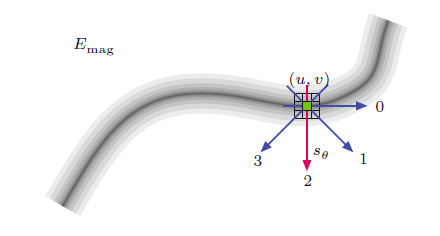
\includegraphics[width=0.6\linewidth]{images/CannyEdgeLocalization}
		\caption[Edge-Localization]{Edge-Localization}
		\label{fig:cannyedgelocalization}
	\end{figure}
	Operate over the magnitude-image:\newline
	Null every value that is not a local-maximum in any direction 
\end{frame}

\begin{frame}
	\frametitle{Canny-Edge}
	\framesubtitle{Hysteresis Thresholding}
	\begin{columns}
		\begin{column}{0.6\textwidth}
			\begin{enumerate}
				\item Find points with $E \geq t_1$
				\item Add Every Neighboor with $E \geq t_2$
				\item Repeat $2$ until image is processed 
			\end{enumerate}
		\end{column}
		\begin{column}{0.4\textwidth}
			\begin{figure}
				\centering
				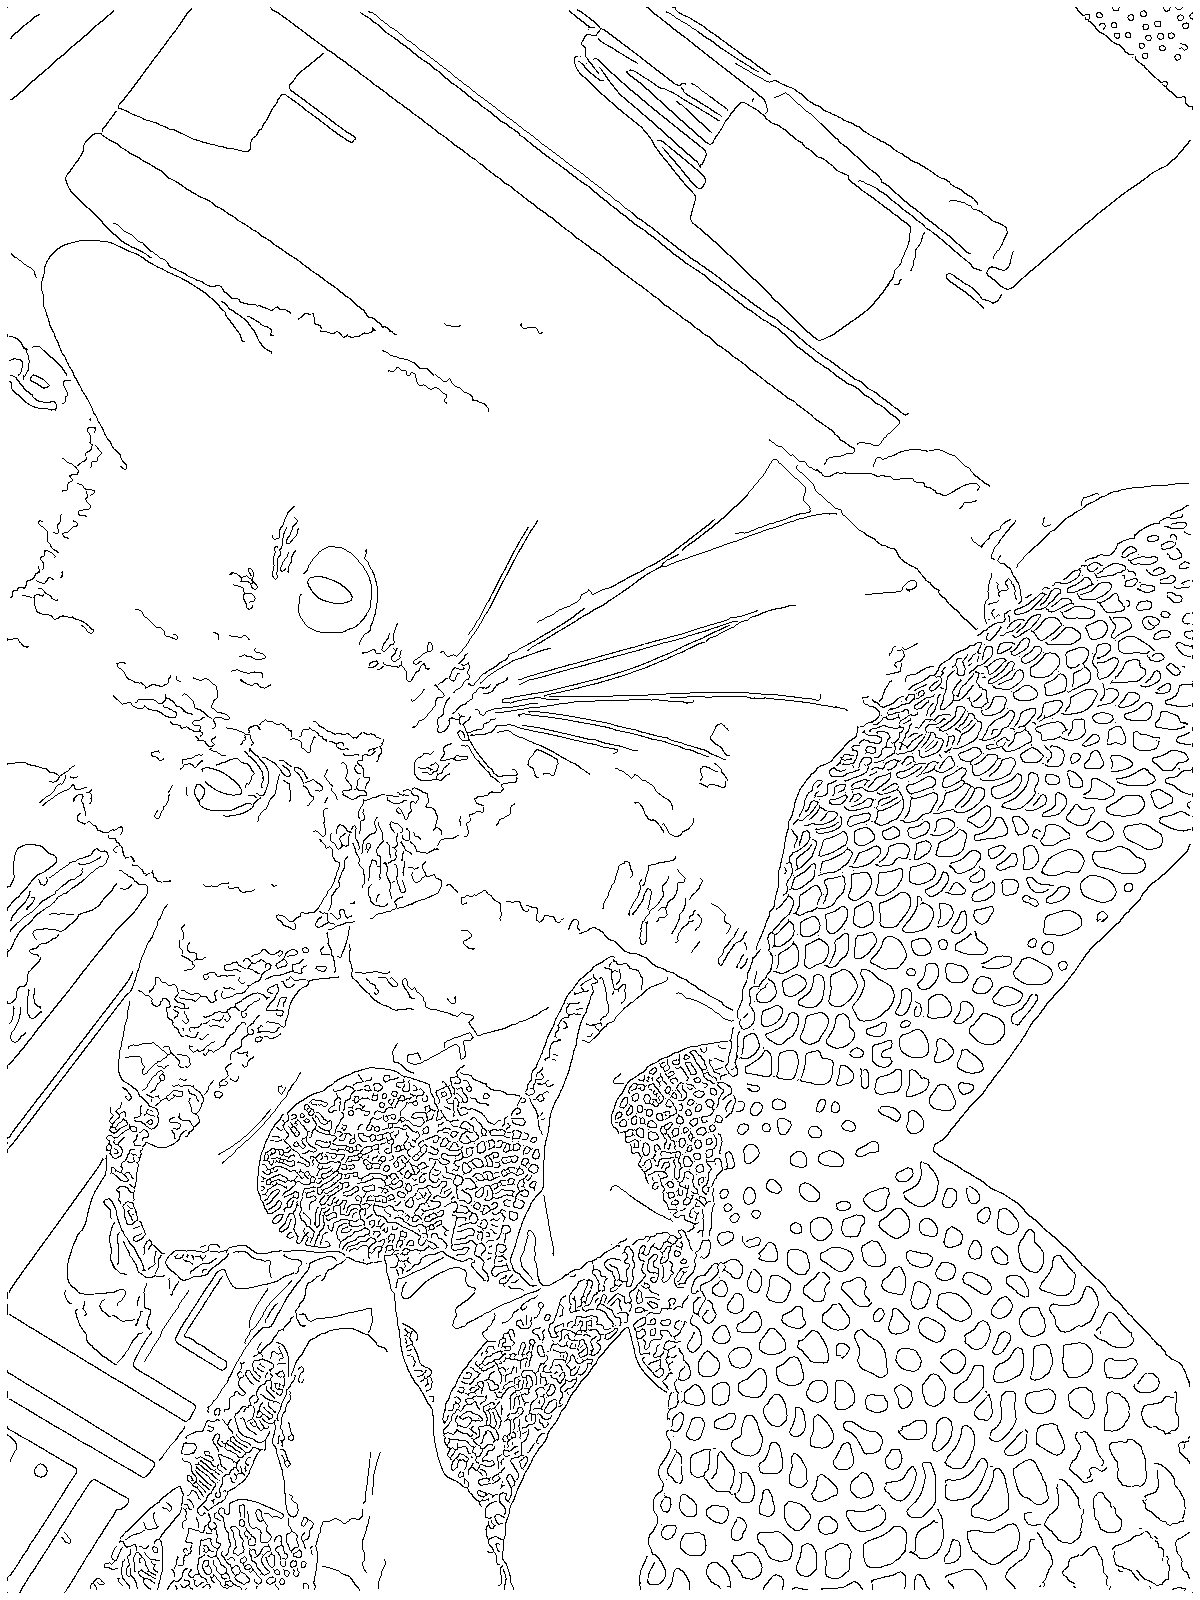
\includegraphics[width=0.9\textwidth]{images/KadseCanny}
				\caption[Canny-Edge Felix\footnote{Took ~30 seconds for Felix}]{Canny-Edge Felix}
				\label{fig:kadsecanny}
			\end{figure}	
		\end{column}
	\end{columns}
\end{frame}
\section{Edge Sharpening}
\begin{frame}
	\frametitle{Laplacian-Filter}
	\framesubtitle{Concept}
	\begin{columns}
		\begin{column}{0.5\textwidth}
			Idea: Alter \textit{steep} imagepoints \newline
			~\newline
			$\hat{f}(x)= f(x) + \omega \cdot f''(x)$ \newline
			~\newline
			Where $\omega$ is a weight for alternation, $f(x)$ is the image function
		\end{column}
		\begin{column}{0.5\textwidth}
			\begin{figure}
				\centering
				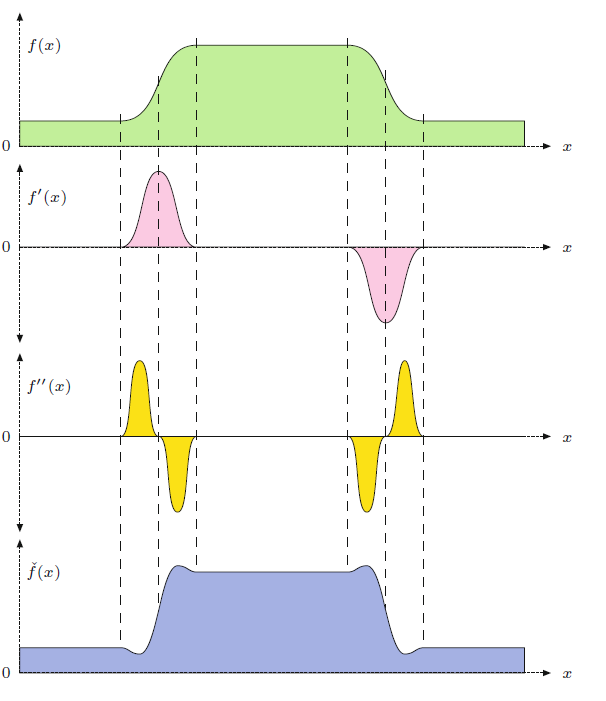
\includegraphics[width=0.8\linewidth]{images/Laplacian}
				\caption[Laplacian Plot]{Applying the Laplacian-Filter}
				\label{fig:laplacian}
			\end{figure}
		\end{column}
	\end{columns}
\end{frame}
\begin{frame}
	\frametitle{Laplacian-Filter}
	\framesubtitle{Implementation}

		Laplacian Operator: $(\nabla^2f)(x,y) = \dfrac{\partial^2f}{\partial^2x}(x,y) +\dfrac{\partial^2f}{\partial^2y}(x,y)$
		~\newline Expressed as filters: 
	\begin{center}
		~\newline ~\newline $\dfrac{\partial^2f}{\partial^2x}(x,y) \approx \begin{bmatrix} 1 & -2 & 1 \end{bmatrix}, \dfrac{\partial^2f}{\partial^2y}(x,y) \approx \begin{bmatrix} 1 \\ -2 \\ 1 \end{bmatrix}$ 
		~\newline ~\newline ~\newline ~\newline
		$\Rightarrow H^L \approx \begin{bmatrix} 0 & 1 & 0 \\ 1 & -4 & 1 \\ 0 & 1 & 0 \end{bmatrix}$
	\end{center}
\end{frame}
\begin{frame}
	\frametitle{Laplacian-Filter}
	\framesubtitle{Variants and Example}
	\begin{columns}
		\begin{column}{0.5\textwidth}
			common variants: ~\newline ~\newline
			$H^L \approx \begin{bmatrix} 1 & 1 & 1\\ 1 & -8 & 1 \\ 1 & 1 & 1 \end{bmatrix}$
			
			~\newline ~\newline
			$H^L \approx \begin{bmatrix} 1 & 2 & 1\\2 & -12 & 2 \\ 1 & 2 & 1 \end{bmatrix}$
			
		\end{column}
		\begin{column}{0.5\textwidth}
			\begin{figure}
				\centering
				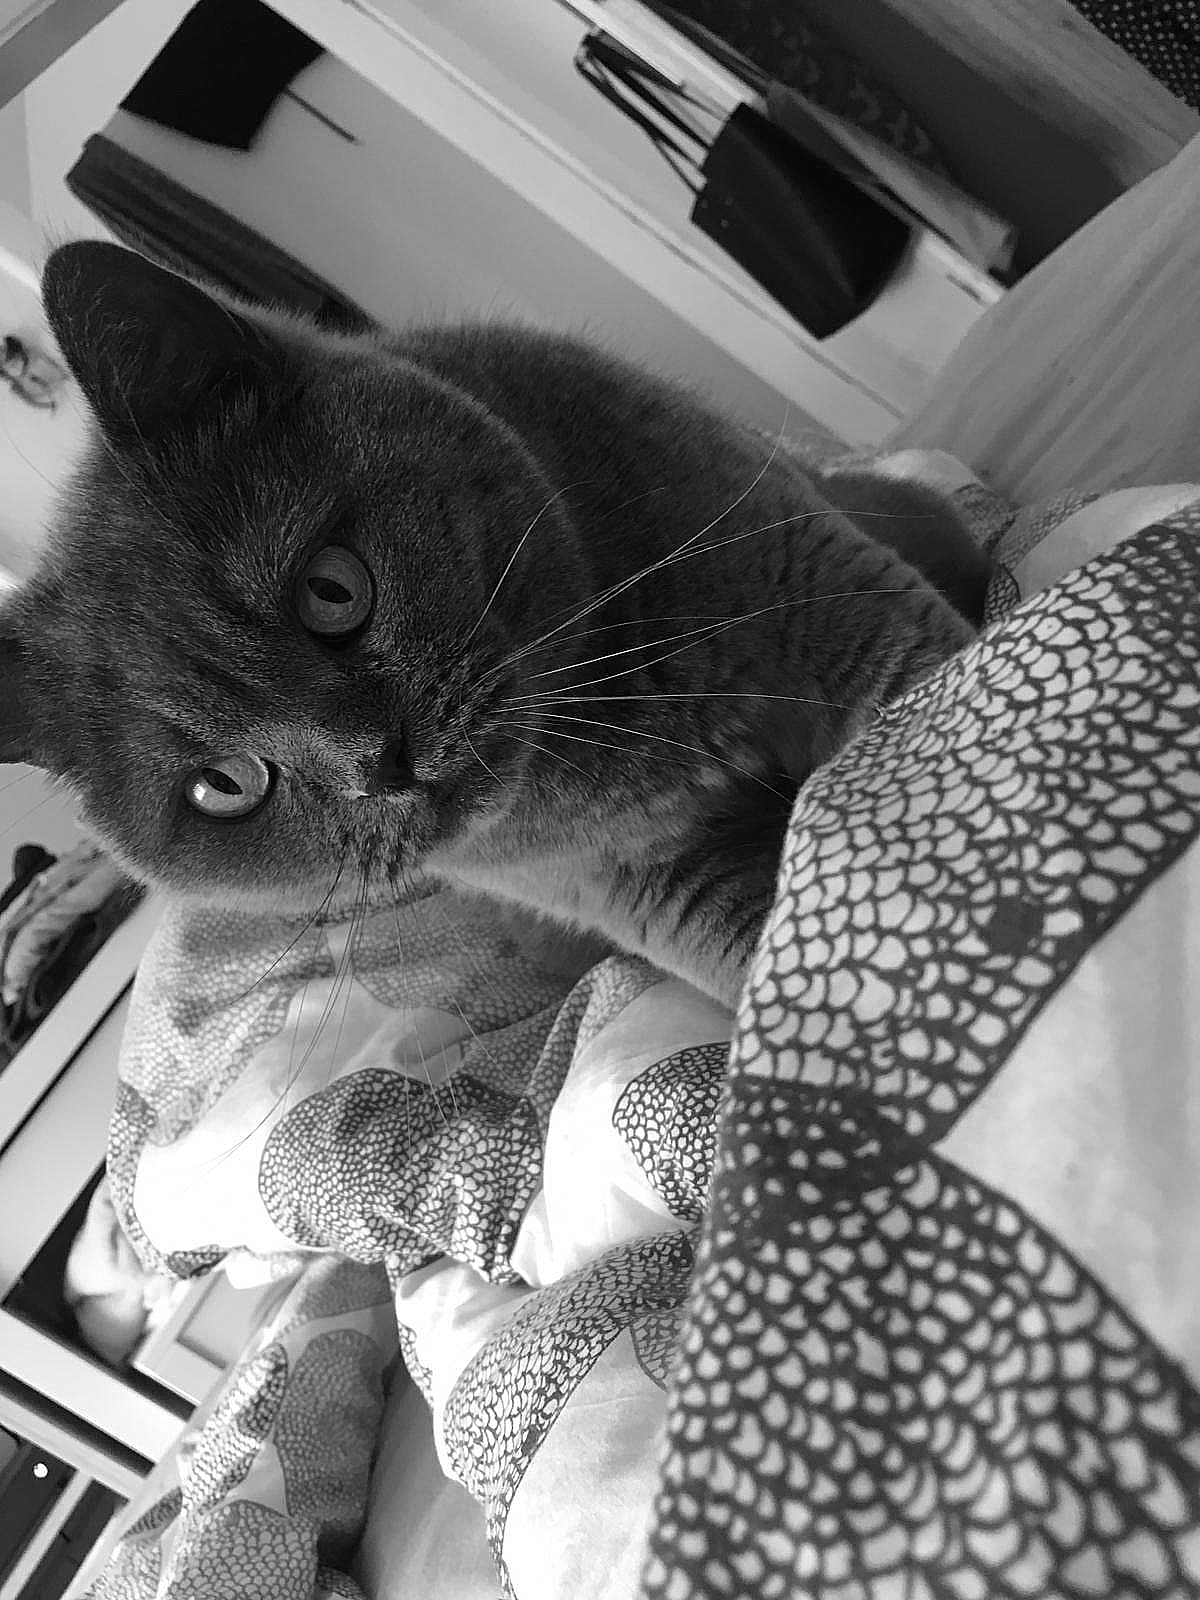
\includegraphics[width=0.7\linewidth]{images/KadseLaplace}
				\caption[FelixLaplace]{Laplacian Filter applied to Felix}
				\label{fig:kadselaplace}
			\end{figure}
		\end{column}
	\end{columns}
\end{frame}
\begin{frame}
	\frametitle{Unsharp Masking (USM)}
	\framesubtitle{Concept}
	\begin{large}
	\begin{enumerate}
		\item produce a smoothed version of the image
		\item subtract the smoothed version from original \newline $\rightarrow$ \textbf{mask} of \textit{sharp} points
		\item add the mask with a weight $\alpha$ to original image
	\end{enumerate}
\end{large}
~\newline ~\newline  ~\newline  
	Any smoothing-filter can be used, but gaussian filters are common \newline
	Notable:
	\begin{itemize}
		\item highly adaptable through exchangeable filters and $\alpha$
		\item Laplacian filters are a implementation of USM with very simple smoothing
		\item vulnerable to \textit{boost} noise, therefore often combined with a threshhold
	\end{itemize}
\end{frame}
